\documentclass{beamer}
\usepackage[latin1]{inputenc}

\usetheme{Madrid}
\usecolortheme{default}
\usepackage{amsmath}
\usepackage{amssymb,amsfonts,amsthm}
\usepackage{txfonts}
\usepackage{tkz-euclide}
\usepackage{listings}
\usepackage{adjustbox}
\usepackage{array}
\usepackage{tabularx}
\usepackage{gvv}
\usepackage{lmodern}
\usepackage{circuitikz}
\usepackage{tikz}
\usepackage{graphicx}
\usepackage{gensymb}
\usepackage{physics}

\setbeamertemplate{page number in head/foot}[totalframenumber]

\usepackage{tcolorbox}
\tcbuselibrary{minted,breakable,xparse,skins}



\definecolor{bg}{gray}{0.95}
\DeclareTCBListing{mintedbox}{O{}m!O{}}{%
  breakable=true,
  listing engine=minted,
  listing only,
  minted language=#2,
  minted style=default,
  minted options={%
    linenos,
    gobble=0,
    breaklines=true,
    breakafter=,,
    fontsize=\small,
    numbersep=8pt,
    #1},
  boxsep=0pt,
  left skip=0pt,
  right skip=0pt,
  left=25pt,
  right=0pt,
  top=3pt,
  bottom=3pt,
  arc=5pt,
  leftrule=0pt,
  rightrule=0pt,
  bottomrule=2pt,
  toprule=2pt,
  colback=bg,
  colframe=orange!70,
  enhanced,
  overlay={%
    \begin{tcbclipinterior}
    \fill[orange!20!white] (frame.south west) rectangle ([xshift=20pt]frame.north west);
    \end{tcbclipinterior}},
  #3,
}
\lstset{
    language=C,
    basicstyle=\ttfamily\small,
    keywordstyle=\color{blue},
    stringstyle=\color{orange},
    commentstyle=\color{green!60!black},
    numbers=left,
    numberstyle=\tiny\color{gray},
    breaklines=true,
    showstringspaces=false,
}
\title{4.3.12}
\date{12th september, 2025}
\author{Vishwambhar - EE25BTECH11025}

\begin{document}

\frame{\titlepage}
\begin{frame}{Question}
Check which of the following are solutions of the equation $x-2y=4$ and which are not\\
\begin{enumerate}
    \item $\brak{0,2}$
    \item $\brak{2,0}$
    \item $\brak{4,0}$
    \item $\brak{\sqrt{2},4\sqrt{2}}$
    \item $\brak{1,1}$
\end{enumerate}
\end{frame}

\begin{frame}{Given}
Given line equation can be written as:
\begin{align}
    \vec{n}^\top\vec{x}=c
\end{align}

where $\vec{n}=\myvec{1\\-2}$, $\vec{x}=\myvec{x\\y}$ and $c=4$.\\
\end{frame}

\begin{frame}{Checking}
Checking whether a point lies on the line or not by substituting given vectors in (1):
\begin{align}
    \vec{x}_1=\myvec{0\\2}, \vec{x}_2=\myvec{2\\0}, \vec{x}_3=\myvec{4\\0}, \vec{x}_4=\myvec{\sqrt{2}\\4\sqrt{2}}, \vec{x}_5=\myvec{1\\1}\\
    \vec{n}^\top\myvec{\vec{x}_1&\vec{x}_2&\vec{x}_3&\vec{x}_4&\vec{x}_5}=\myvec{c_1&c_2&c_3&c_4&c_5}\\
    \myvec{1&-2}\myvec{0&2&4&\sqrt{2}&1\\2&0&0&4\sqrt{2}&1}=\myvec{-4&2&4&-7\sqrt{2}&-1}\\
\end{align}

\end{frame}

\begin{frame}{Conclusion}
Conclusion:\\

The point which lies on the line is only option (3).
\end{frame}

\begin{frame}[fragile]
    \frametitle{C Code}
    \begin{lstlisting}
#include <stdio.h>

#define size 2

double n[size], v1[size], v2[size], v3[size], v4[size], v5[size];

void insert_vector(int index, double vec[size]){
    double *target;
    switch (index){
        case 0: target = n; break;
        case 1: target = v1; break;
        case 2: target = v2; break;
        case 3: target = v3; break;
        case 4: target = v4; break;
        case 5: target = v5; break;
    }
    for (int i=0; i<size; i++){
        target[i] = vec[i];
    }
}
    \end{lstlisting}
\end{frame}

\begin{frame}[fragile]
    \frametitle{C Code}
    \begin{lstlisting}
double* get_vector(int index){
    switch (index){
        case 0: return n;
        case 1: return v1;
        case 2: return v2;
        case 3: return v3;
        case 4: return v4;
        case 5: return v5;
        default: return NULL;
    }
}
    \end{lstlisting}
\end{frame}

\begin{frame}[fragile]
    \frametitle{Python Code 1}
    \begin{lstlisting}
import matplotlib.pyplot as plt
import numpy as np
import math

x = np.linspace(-6, 10, 100)   
y = x/2 - 2
X = [0, 2, 4, 1, math.sqrt(2) ]
Y = [2, 0, 0, 1, 4*math.sqrt(2)]

plt.plot(x, y, 'r-', label="x-2y=4")
plt.plot(X, Y, 'ko')  

plt.text(8.17, 1.76, "x-2y=4", fontsize=12, color='black')

for i in range(len(X)-1):
    plt.text(X[i]+0.1, Y[i]+0.1, f"({X[i]},{Y[i]})", fontsize=10, color='black')
    \end{lstlisting}
\end{frame}

\begin{frame}[fragile]
    \frametitle{Python Code 1}
    \begin{lstlisting}
plt.axvline(x=0, color='k', linewidth=1.5)

plt.axhline(y=0, color='k', linewidth=1.5)
plt.title("Plot of the given line and points")
plt.xlabel("X-axis")
plt.ylabel("Y-axis")
plt.axis('equal')
plt.grid(True)
plt.savefig("../figs/plot.png")
plt.show()
    \end{lstlisting}
\end{frame}

\begin{frame}[fragile]
    \frametitle{Python Code 2}
    \begin{lstlisting}
import ctypes
import numpy as np
import math

lib = ctypes.CDLL("./problem.so")

lib.insert_vector.argtypes = (ctypes.c_int, ctypes.POINTER(ctypes.c_double))
lib.insert_vector.restype = None

lib.get_vector.argtypes = (ctypes.c_int,)
lib.get_vector.restype = ctypes.POINTER(ctypes.c_double)

    \end{lstlisting}
\end{frame}

\begin{frame}[fragile]
    \frametitle{Python Code 2}
    \begin{lstlisting}
    vectors = [
    [1, -2],
    [0, 2],
    [2, 0],
    [4, 0],
    [math.sqrt(2), 4*math.sqrt(2)],
    [1, 1],
]
for i, vec in enumerate(vectors):
    arr = (ctypes.c_double * 2)(*vec)
    lib.insert_vector(i, arr)

def get_vector(i):
    ptr = lib.get_vector(i)
    return np.ctypeslib.as_array(ptr, shape=(2, ))

all_vectors = [get_vector(i) for i in range(0, 6)]
    \end{lstlisting}
\end{frame}

\begin{frame}[fragile]
    \frametitle{Python Code 2}
    \begin{lstlisting}
n = get_vector(0)

for i in range(1, 6):
    v = get_vector(i)
    v_T = v.T
    res = n@v_T
    if(res==4):
        print(f"option ({i}) lies on the given line.")
    else:
        print(f"option ({i}) does not lie on the given line.") 
    \end{lstlisting}
\end{frame}





\begin{frame}{Plot}
    \begin{figure}
        \centering
        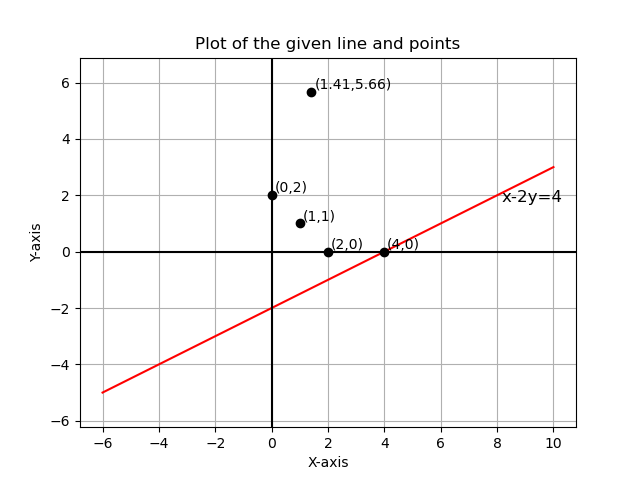
\includegraphics[width=0.5\columnwidth]{../figs/plot.png}
        \caption{Plot of given line and points}
        \label{fig:fig}
    \end{figure}
\end{frame}




\end{document}